\subsection{Code Metrics}
This project details which measures where put in place in order to ensure that the quality of the plugin followed a hight standard. This was important since the goal was not to develop a proof of concept, but a production ready solution. For this project it was decided to use SonarQube, a static code metrics analyzer to gain insight into the quality of the work done.\newline
During the whole development, SonarQube was always part of the continuous integration process. Due to this, it was clear in which direction code quality developed after every commit. Very serious vulnerabilities also triggered messages being sent, so that a quick reaction was possible. \newline
All standard configurations of SonarQube for Typescript were let be, because in this configuration SonarQube is the strictest. This meant that the coder base was subject to 117 rules regarding the code quality analysis. The only exception that had to be done was that a class called Symbol was written during the implementation. SonarQube kept getting this class confused with the built in class symbol, the usage of which is discouraged. To not be subject to false positives, it was decided to disable this rule.\newline
Following, some key metrics delivered by SonarQube are given.\newline
\begin{figure}[H]
	\centering
	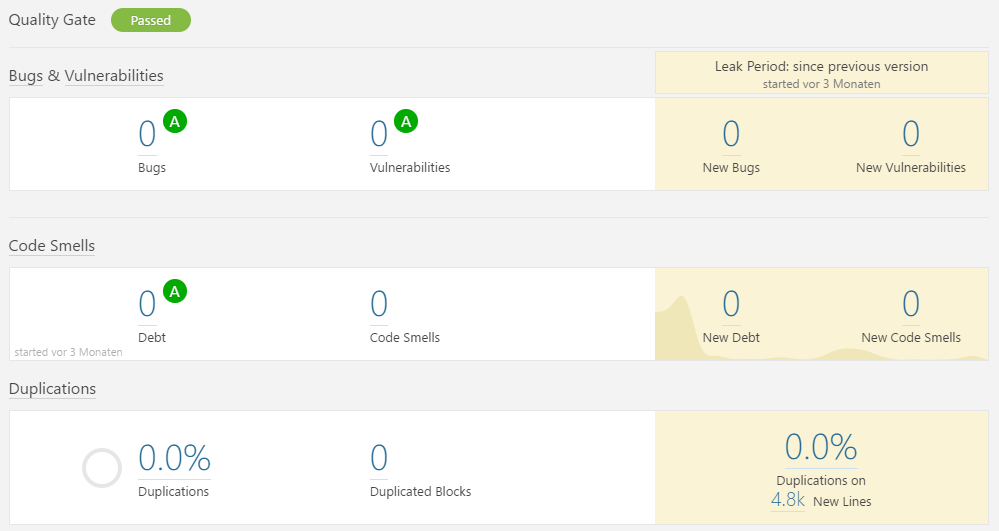
\includegraphics[width=1\textwidth]{img/sonarAll}
	\caption{Overview of the analysis}
	\label{fig:sonarQubeOverview}
\end{figure}
In the complete overview of the project, it can be seen that SonarQube does not detect any Bugs or Vulnerabilities in the project. Starting from about the middle of the project, all code smells that SonarQube can detect could be avoided, this due to continuous adaption of the design and the review processes. During the development a key concern was to avoid code duplication. This was done through design reviews and IDE-Tools. The analysis shows that these efforts were fruitful.\newline
The only negative point in the way SonarQube could be integrated is that SonarQube seems not to be able to detect code coverage generated by application of Visual Studio Code's testing framework. After some time spent trying to make this work, it was decided to mitigate the missing information about code coverage by writing conservative test specifications which can be found in the API documentation.\newline
\begin{figure}[H]
	\centering
	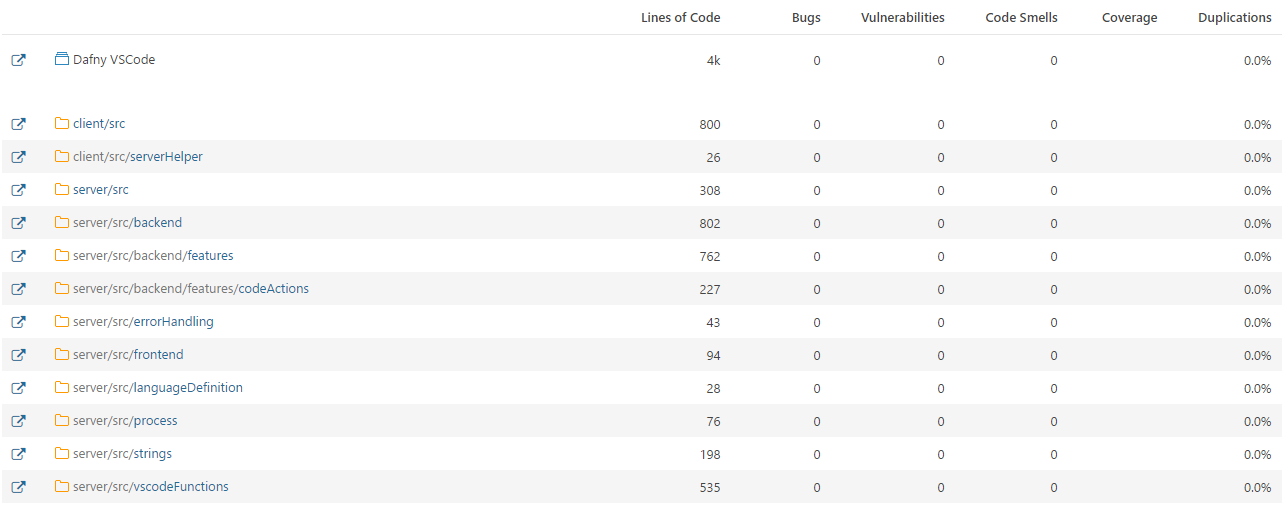
\includegraphics[width=1\textwidth]{img/sonarSize}
	\caption{Overview of the code base size}
	\label{fig:sonarQubeSizeOverview}
\end{figure}
In the overview regarding size it can be seen that the project consists of about 4'000 lines of code. The major part thereof not surprisingly is situated in the language server part of the project. The client part consists of about 800 lines of code, but most of this is due to the tests defined here. The actual logic in the client is only about 100 lines of code, underlining the portability of this project.\newline
\begin{figure}[H]
	\centering
	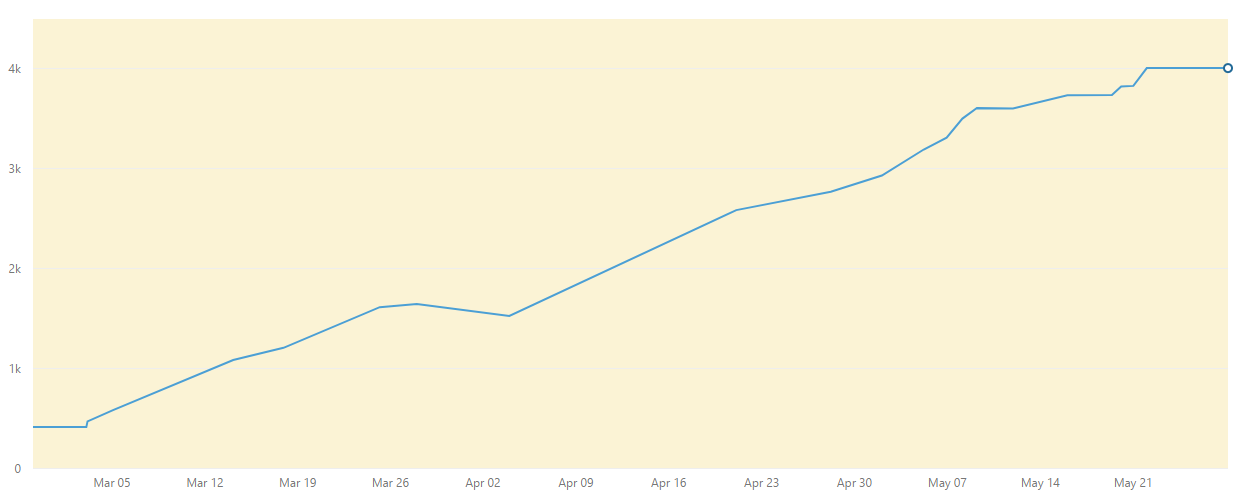
\includegraphics[width=1\textwidth]{img/sonarTime}
	\caption{Overview the amount of code written over time}
	\label{fig:sonarQubeTimeOverview}
\end{figure}
As can be seen in the overview of code being added over the time, the amount of code written steadily progressed. Through refactorings and improvements regarding the design the size was also reduced again from time to time, but new features were always quickly developed.\newline
Concluding it can be said that the analysis done by SonarQube ascertains that the project is subject to a high quality standard. The high maintainability rating and the absence of code duplication is a good indicator that this project can be continue to be developed without problems. Additionally, all bugs, code smells and vulnerabilities that SonarQube can detect could be detected form early on in the project. It has to be said that the analysis of Typescript code is not quite as sophisticated as the one it provides for Java or C\#, as for instance complexity is not analyzed in detail. However, the analysis provided lays a good basis for reasoning about the quality of the project.  
